\chapter{Approach}\label{sec:approach}

We propose two different approaches to relocalization: first, a local approaches based on the PTAM implementation, where two steps are performed. The first step has been named \textit{Place Finder} and the second \textit{Real Pose Recognition}. Multiple methods will be proposed to solve the second step. Then, on the other side, a global approach will be proposed. In this case machine learning methods (\textit{ferns}) will be used to recognize points in space.

\section{PTAM method}
\label{sec:ptam_method}

PTAM~\cite{KleinMurray2007} is a VO algorithm based on keyframes and so the relocalization method proposed is based on keyframes as well. Every keyframe has associated with a camera pose that will be used to relocalize. During the relocalization there are two steps involved. We called the first step \textit{Place Finder} and the second \textit{Real Pose Finder}.

\subsection{Place Finder}
\label{ssub:place_recognition}

During this step, the algorithm tries to find the keyframe image most similar to the last acquired image. The pose associated with the most similar keyframe is used as an initial rough estimation of the current pose. The similarity score should be resistant to view point because the new acquired image will, most probably, never be taken from the same pose as any of the keyframes. Also it should be fast to compute.\\

The used similarity score is the Cross Correlation between images meaning the sum of the squared error between two zero-mean images. To make to computation faster both images are resized become $40\times30$. Then, to make the images more resistant to view point changes it is blurred with a $3\times3$ Gaussian kernel with $\sigma=2.5$. The resulting image is a resized, blurred and zero-mean image called \textit{small-blurry-image}.\\

During the normal map building pipeline this image is computed and stored every time a new keyframe is added to the map. And then, during the relocalization, the sum of squared difference between every stored \textit{small-blurry-image} and the last acquired frame is computed, the corss correlation measure, to find the most similar keyframe, which is then use its pose as an initial estimation of the current camera pose.\\

\subsubsection{Method validation}
\label{ssub:cc_method_validation}

To evaluate the method the real distance between two frames is going to be compared with the Cross Correlation value described above. Far away frames should be dissimilar and close by frames should be more similar and have a lower CC value. In Figure~\ref{fig:real_distance_confusion_matrix} can be seen the pair distances between image using the real pose while in Figure~\ref{fig:CC_confusion_matrix} there is the approximated pair distances using the CC value as distance. It can be seen that they have a similar distribution. Also the correlation of 0.4337 shows numerically its relation.\\

\begin{figure}
  \begin{subfigure}[b]{0.50\linewidth}
          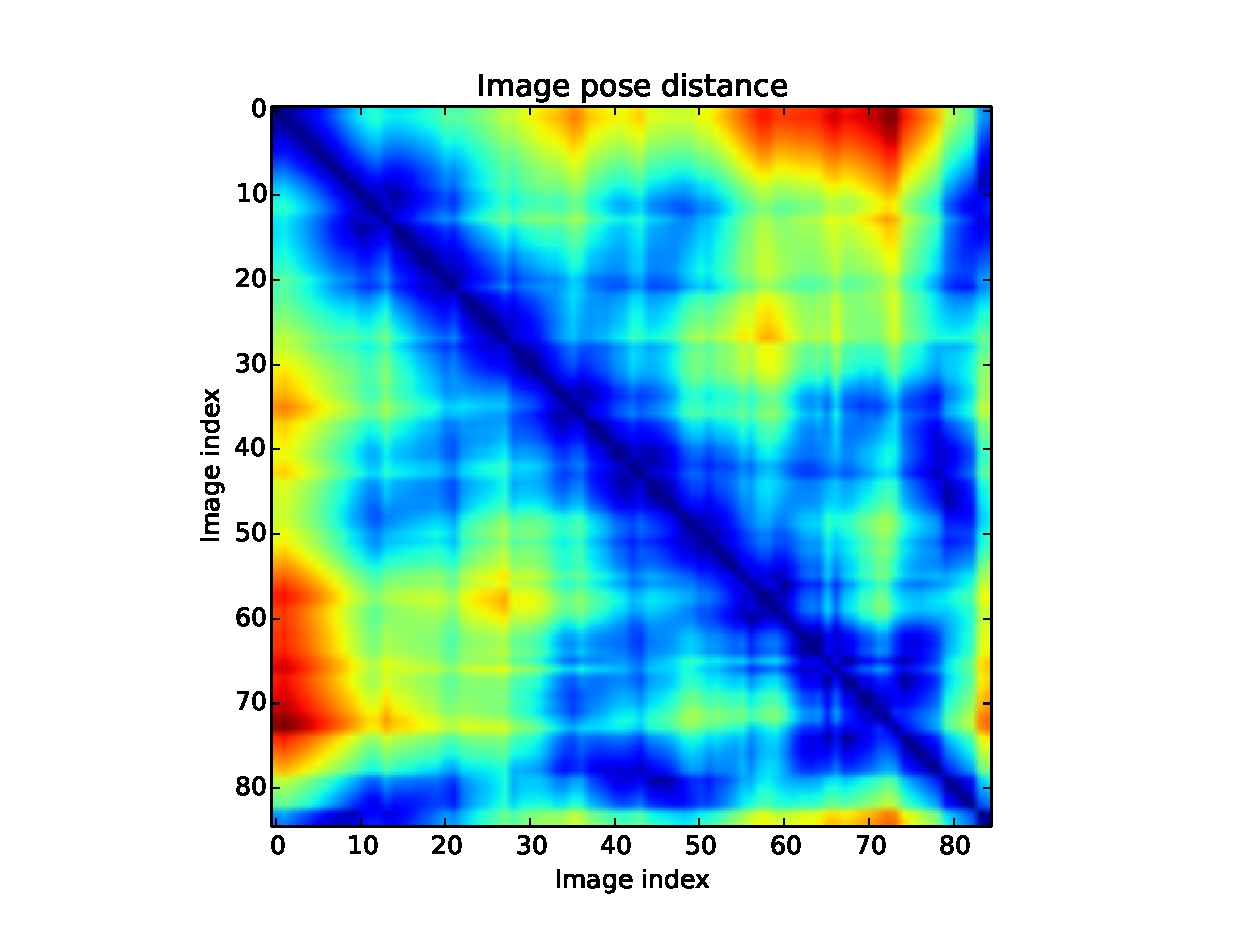
\includegraphics[width=\linewidth]{img/demo_1_1_CC_real_similarity_matrix.eps}
          \caption{Image to image real distance between the keyframe pose}                
          \label{fig:real_distance_confusion_matrix}
  \end{subfigure}   
  \quad
  \begin{subfigure}[b]{0.50\linewidth}
         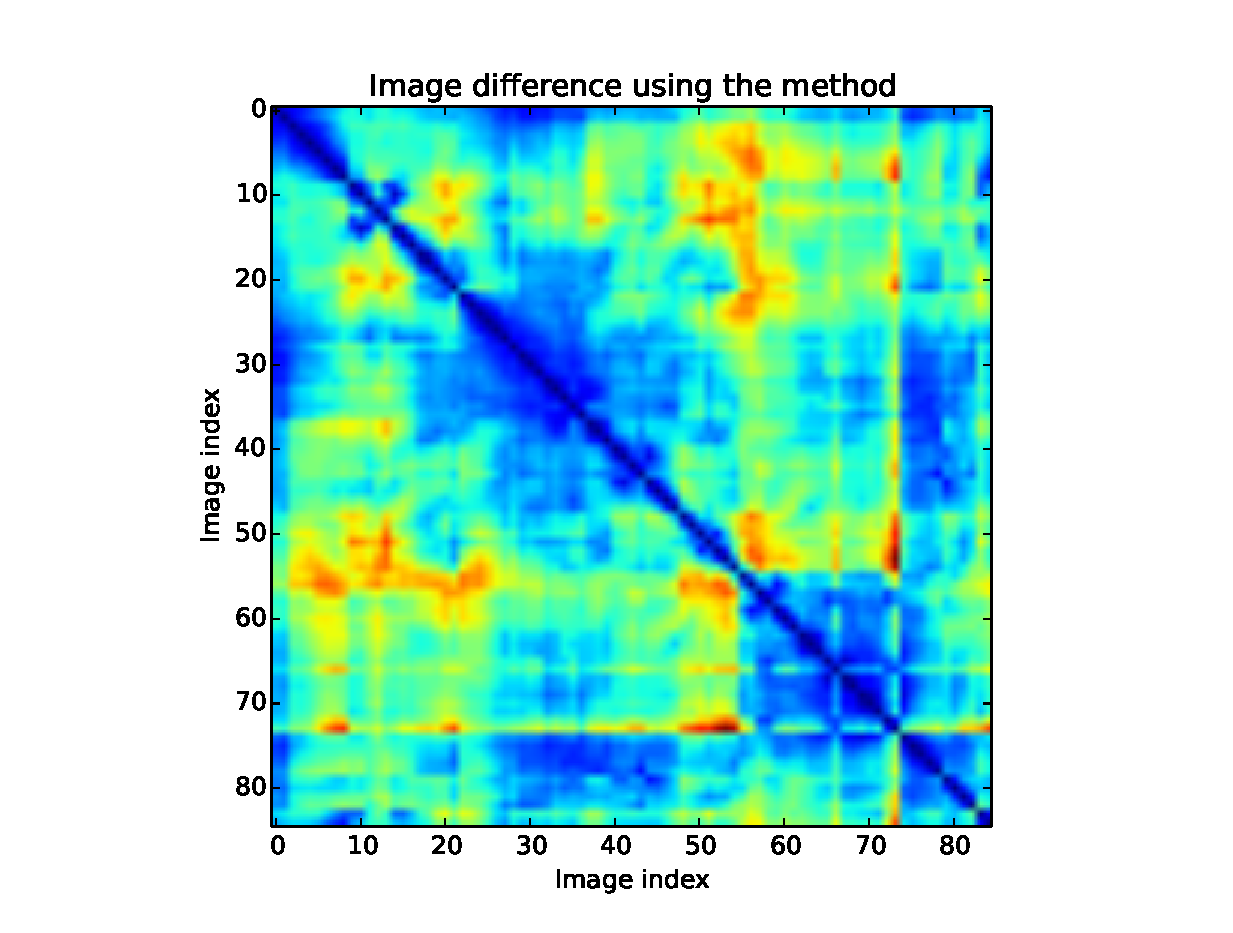
\includegraphics[width=\linewidth]{img/demo_1_1_CC_CC_similarity_matrix.eps}
         \caption{Image to image distance approximated using the Cross Correlation value}                
         \label{fig:CC_confusion_matrix}
  \end{subfigure}
  \caption{}
\end{figure}


Finally, to show that this method can be used, for every image the most similar, in CC seance, image was taken being it actually the  $K$th closest image. Ideally the most similar image should always be the closest image. In Figure~\ref{fig:K_closest} there is the count of occurrences of each $K$. It can be seen that most images resolve to the first or second closest image using this method.\\

\begin{figure}[!htbp]
  \centering
  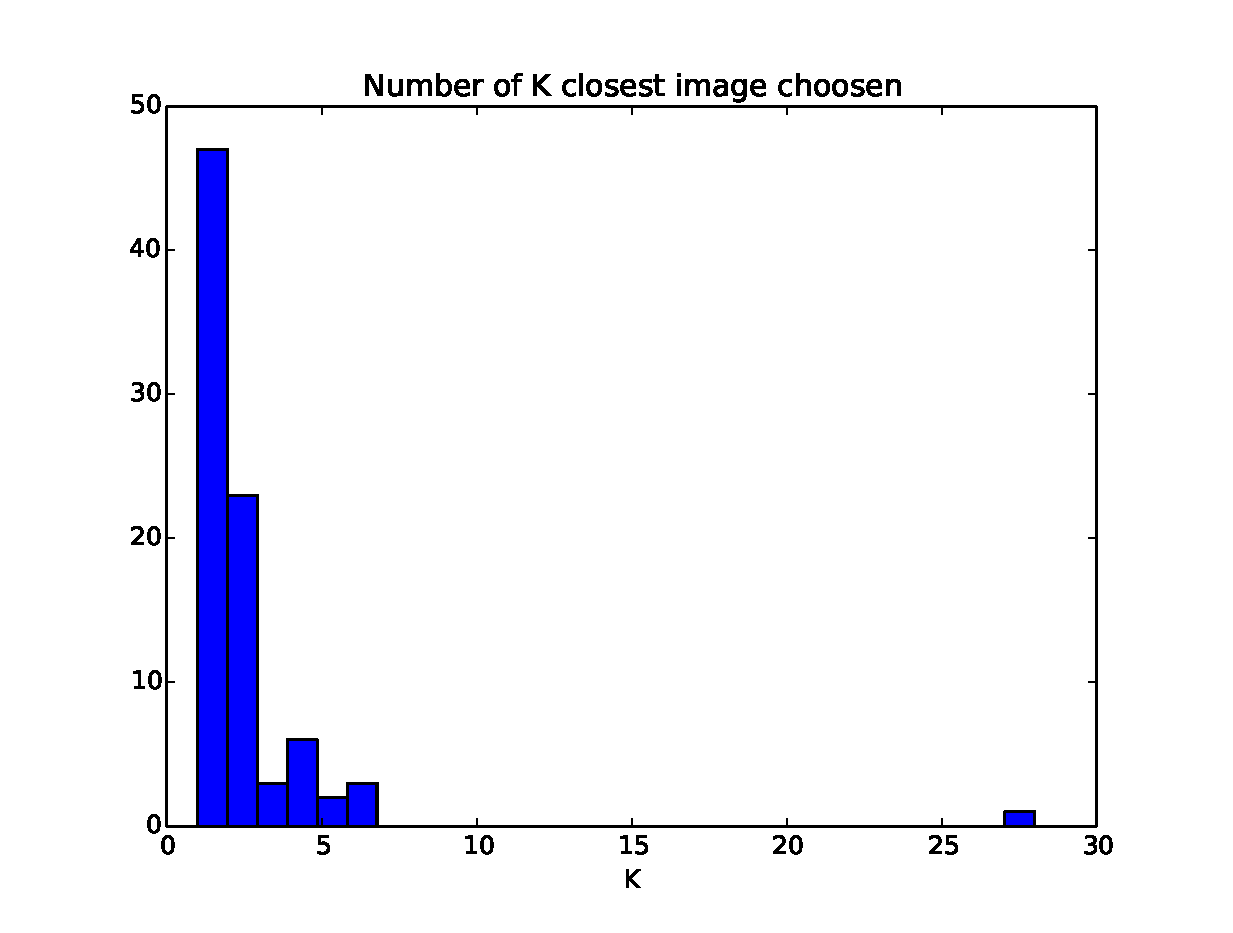
\includegraphics[width=9cm]{img/demo_1_1_CC_choose_distribution.eps}
  \caption{Distribution of closest chosen images using CC}
  \label{fig:K_closest}
\end{figure}


\begin{figure}[!htpb]
  \centering
  \begin{subfigure}[b]{11cm}
    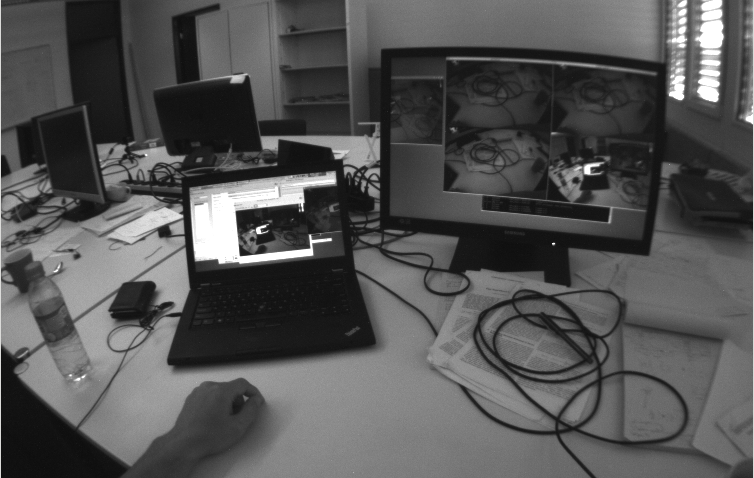
\includegraphics[width=\linewidth]{img/query_1.png}
    \caption{Query image}
    \label{fig:query_1}
  \end{subfigure}

  \begin{subfigure}[b]{11cm}
    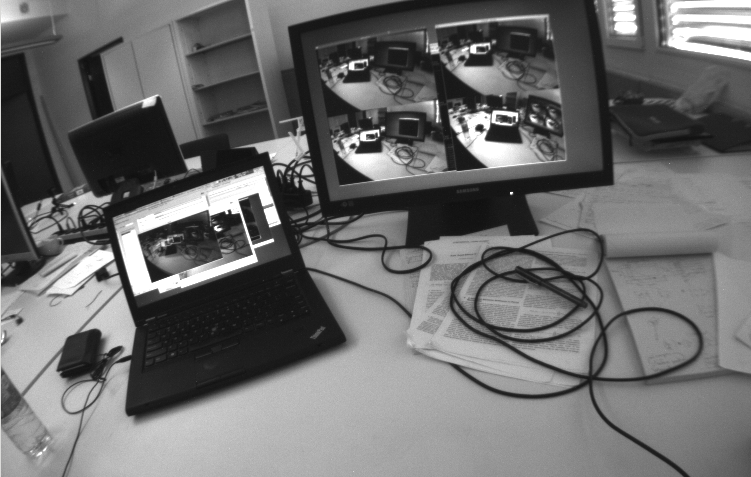
\includegraphics[width=\linewidth]{img/best_match_1.png}
    \caption{Found closest image}
    \label{fig:best_match_1}
  \end{subfigure}
  \caption{}
  \label{fig:cc_example}
\end{figure}


In Figure~\ref{fig:cc_example} demonstrates what the algorithm would return for a given query image for which there is no pose information available. Figure~\ref{fig:query_1} is the image seen by the camera at the moment of the relocalization and~\ref{fig:best_match_1} is what the system found to be the most similar, closest, image using the cross correlation procedure explained previously. In this case the to image's camera pose are not the same, but they should be similar enough in order to find the difference in posterior steps.\\

\subsection{Real Pose Finder}
\label{sub:real_pose_finder}

The second step of the relocalization algorithm from PTAM tries to refine the pose of the found to be most similar keyframe to explain the current pose of the camera. During this step, in the implementation from PTAM, only rotations are corrected. An image alignment through optimization algorithm (ESM~\cite{lovegrove2012parametric}) is used to find the $SE(2)$ transformation between the two and then an other minimization is performed to find a transformation in the world frame.\\

\subsubsection{Image alignment}
\label{ssub:image_alignment}

The Extended Second order Minimization algorithm (ESM) is based on the algorithm proposed by Lucas and Kanade \cite{Baker2004} in 1981. The goal of both algorithms is to align one template image $T$ to a different input image $I$ through a parametrised warping function. \\

With this goal an error function is defined on which the Gauss-Newton or Levenberg-Marquardt schemes can be applied. The error is the squared difference between the template image and the warped input image

\begin{equation}
  \sum_x [I(W(x;p)) - T(x)]^2
\end{equation}

The warping function is going to be in $SE(2)$, that is, translation and rotation of the image.

\begin{equation}
  W(x;p) = 
  \begin{bmatrix}
    cos (\alpha) & sin(\alpha) & t_x\\
    -sin(\alpha) & cos(\alpha) & t_y\\
    0 & 0 & 1 \\
  \end{bmatrix}
  \begin{bmatrix} x \\ y \\ 1 \end{bmatrix}
    =
  \begin{bmatrix}
    xcos(\alpha) + y sin(\alpha) + t_x \\
    -x sin(\alpha) + y cos(\alpha) + t_y \\
  \end{bmatrix}
  \label{eq:se2_warp_function}
\end{equation}

where $p = \begin{pmatrix} \alpha , t_x , t_y \end{pmatrix}$ are the $SE(2)$ parameters and $x = \begin{pmatrix} x , y \end{pmatrix}$ is a pixel coordinate.\\

  The algorithm assumes that a current estimate of $p$ exists and iteratively tries improves it by increments $\Delta p$. On every  iteration equation~\ref{eq:delta_error} is solved on $\Delta p$ and then it is used to update $p$ as in~\ref{eq:p_update}

\begin{equation}
  \sum_x [I(W(x;p + \Delta p)) - T(x)]^2
  \label{eq:delta_error}
\end{equation}

\begin{equation}
  p \leftarrow p + \Delta p
  \label{eq:p_update}
\end{equation}

To solve question~\ref{eq:delta_error}  it first needs to be linearised. With this goal, a first Taylor expansion on $I(W(x:p + \Delta p))$ is carried on leading to

\begin{equation}
\sum_x [I(W(x;p)) + \nabla I \frac{\parial W}{\partial p} \Delta p - T(x)]^2
\end{equation}

where $\nabla I$ is the gradient of the input image and $\frac{\partial W}{\partial p}$ is the Jacobian of the warping function. In this case the Jacobian of~\ref{eq:se2_warp_function} is

\begin{equation}
  \frac{\partial W}{\partial p}
  =
  \begin{bmatrix}
    -xsin(\alpha) - ycos(\alpha) & 1 & 0 \\
    xcos(\alpha) - ysin(\alpha) & 0 & 1 \\
  \end{bmatrix}
  \label{eq:se2_jac}
\end{equation}


The solution that minimizes~\ref{eq:delta_error}  on $\Delta p$ can be found in a least squares sense. The equation needs to be derived and then set it equal to zero. The partial derivative of~\ref{eq:delta_error} with respect to $\Delta p$ is:

\begin{equation}
  2 \sum_x \left[\nabla I \frac{\partial W}{\partial p}\right]^T \left[I(W(x;p)) + \nabla I \frac{\partial W}{\partial p} \Delta p - T(x) \right]
  \label{eq:derivated}
\end{equation}

Then, setting~\ref{eq:derivated} equal to zero to find where it is minimized (or maximized) by $\Delta p$ and isolating $\Delta p$ the next closed form solution can be found:

\begin{equation}
  \Delta p = H^{-1} \sum_x \left[\nabla I \frac{\partial W}{\partial p}\right]^T \left[ T(x) - I(W(x;p)) \right]
\end{equation}

Where $H$ is the Gauss-Newton approximation of the Hessian matrix:

\begin{equation}
  H = \sum_x \left[\nabla I \frac{\partial W}{\partial p}\right]^T \left[\nabla I \frac{\partial W}{\partial p}\right]
\end{equation}


The ESM algorithm used in PTAM is very similar to the derived above with the difference that while the Lucas-Kanade takes the gradient from the input image, ESM used both the gradient of the input image and the gradient of the template image and averages them.

\begin{equation}
  \nabla I = \frac{1}{2} \left[\nabla I_t + \nabla I_q \right]
\end{equation}

\begin{equation}
  \textit{steepest descent}\text{ image} = \nabla I \frac{\partial W}{\partial p}
  \label{eq:steepest_image}
\end{equation}

What in~\cite{Baker2004} is referred as \textit{steepest descent} image~\ref{eq:steepest_image} in PTAM and other references is the Jacobian. That is, the gradient of the image multiplied by the Jacobian of the warp function. Taking the used Jacobian \ref{eq:se2_jac} the \textit{steepest descent} image would be

\begin{equation}
  \begin{array}{l l}
  \textit{steepest descent}\text{ pixel} = \begin{bmatrix}  g_x & g_y \end{bmatrix} 
  \begin{bmatrix}
    -xsin(\alpha) - ycos(\alpha) & 1 & 0 \\
    xcos(\alpha) - ysin(\alpha) & 0 & 1 \\
  \end{bmatrix}
  \\ \\=
  \begin{bmatrix}
    g_x(-xsin(\alpha) - ycos(\alpha)) + g_y(xcos(\alpha) - ysin(\alpha)) & g_x & g_y
  \end{bmatrix}
  \\ \\
  \approx
  \begin{bmatrix}
    -y g_x + x g_y & g_x & g_y
  \end{bmatrix}
  \quad \text{when} \quad
  \alpha \approx 0
\end{array}
\end{equation}

During the implementation, $\alpha$ is considered to be close to zero. This way the computation of the trigonometric functions is avoided. This method is first applied to the last level of the scale pyramid roughly aligning the images and then refined with upper levels (used top level is a configuration parameter). \\






\subsubsection{World frame interpretation}
\label{ssub:world_frame_interpretation}

This transformation is not easily interpreted in $SE(3)$, a translation in pixels can mean different things in the world frame depending on the distance to the object. Also, in $SE(3)$ there are three angular degrees of freedom, only. The found transformation can be interpreted in multiple ways in the world frame. In the PTAM implementation it is assumed that the translation will only involve rotations, and so, the next step is the mapping from $SE(2)$ to $SO(3)$. This final found transformation, only including rotations, will actually translate the frame pose because this rotation is not, probability, applied from the origin.\\

A Gauss-Newton minimization algorithm is used to find the $SO(3)$ model that modifies the image in the same way as the found $SE(2)$ model. The minimization is over the $SO(3)$ parameters $\xi$ and the error is expressed as in~\ref{equ:so3_error}

\begin{equation}
  \delta_i(\xi) = T_{SE(2)}u_i - \pi(T_{SO(3)}(\xi) p_i) \qquad \text{where} \quad u_i = \pi(p_i)
  \label{equ:so3_error}
\end{equation}


where $u_i$ is a pixel position (during the implementation $u_0=(5,0)$ and $u_1=(-5,0)$ are used). Also the Jacobian of $\delta$ is needed during the minimization process.

\begin{equation}
  \frac{\partial \delta(\xi)}{\partial \xi} = -\frac{\partial \pi (b)}{\partial b}|_{b=p} \frac{\partial T_{SO(3)}(\xi)}{\partial\xi}|_{\xi=0} \quad p
\end{equation}

with

\begin{equation}
  \frac{\partial \pi(b)}{\partial b} |_{b=p} = \frac{f}{z}
  \begin{bmatrix}
    1 & 0 & -\frac{x}{z} \\
    0 & 1 & -\frac{y}{z}
  \end{bmatrix}
  \qquad \text{where} \quad 
  p = \begin{bmatrix} x \\ y \\ z \end{bmatrix} \quad \text{and} \quad f = \text{focal length}
\end{equation}

\begin{equation}
  \frac{\partial T_{SO(3)}(\xi)}{\partial \xi_k}  = G_k \qquad \text{where} \quad G = \text{$SO(3)$ Generator}
\end{equation}


\subsubsection{Method validation}
\label{ssub:esm_method_validation}

To visualize the results of the different optimization procedures described above, the found transformation has been applied to the image. In the first step, the $SE(2)$ transformation between two image is computed and the transformed image at every step is one of the used variables. In Figure~\ref{fig:se2_transformation_1} can be seen the final transformation found from~\ref{fig:best_match_1} to~\ref{fig:query_1}. In Figure~\ref{fig:se3_error_1} the error of the overplayed images is visualized, there it can be seen that translation and rotation are well corrected but there still is a misalignment caused mostly by a change on scale which is not taken into account during the alignment.\\

\begin{figure}[htpb]
  \centering
  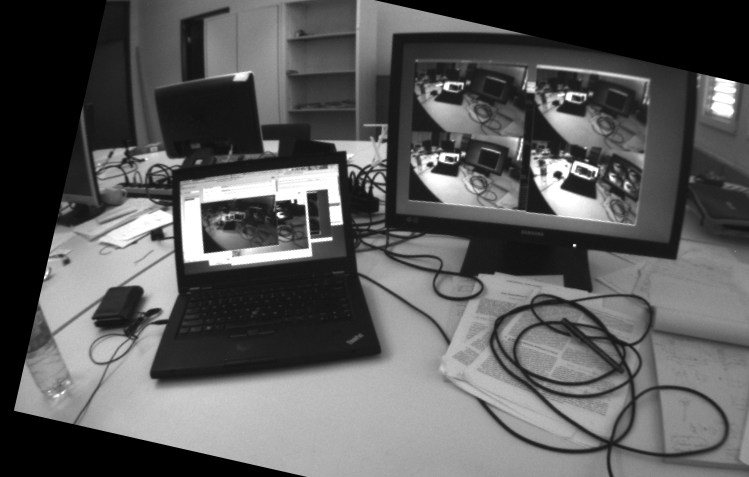
\includegraphics[width=11cm]{img/se2_transformation_1.png}
  \caption{$SE(2)$ transformed image}
  \label{fig:se2_transformation_1}
\end{figure}

On the other side, during the second minimization where a $SO(3)$ translation is found, no image is actually involved, only two pixel coordinates. To generate a visualization of the translation the calibration of image unit plane. Every pixel is unprojected form the image into the image plane, then the transformation is applied to it and finally it is projected back to the image. The result of the described procedure can be seen in Figure~\ref{fig:so3_transformation_1}.\\

\begin{figure}[htpb]
  \centering
  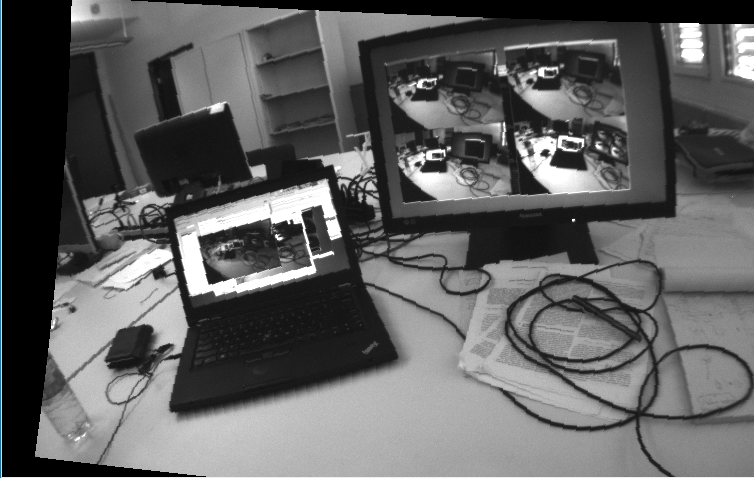
\includegraphics[width=11cm]{img/so3_transformation_1.png}
  \caption{$SO(3)$ transformed image}
  \label{fig:so3_transformation_1}
\end{figure}

\begin{figure}[htpb]
  \centering
  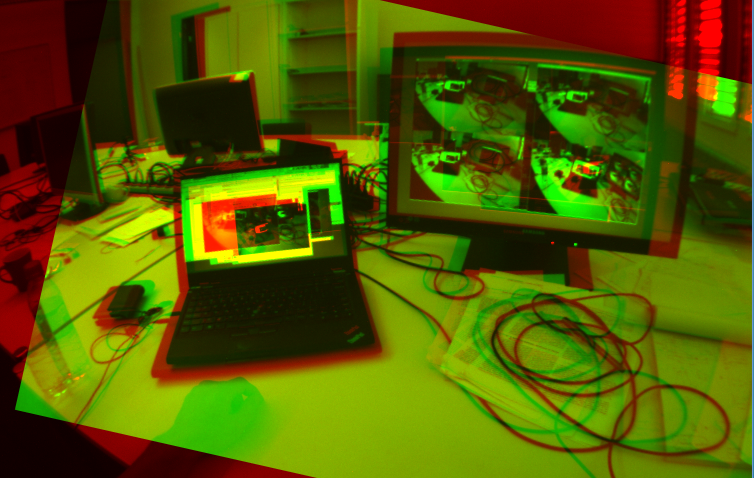
\includegraphics[width=11cm]{img/se2_error_1.png}
  \caption{$SE(2)$ transformation error visualization}
  \label{fig:se3_error_1}
\end{figure}


\subsection{Real Pose Finder Alternative}
\label{sub:real_pose_finder_alternative}

During the mapping of an area the VO algorithm finds landmarks in the world frame which are associated with detected featured points in keyframes (i.e. every featured point in an image is related to a $3D$ position in the world frame). Given a new image, some extracted featured points can be related to a keyframe using descriptor-matching which at the same time are related to world positions. From this information the full 6 DoF translation $SE(3)$ can be computed using the prospective three-point algorithm (P3P).\\

The 3pt algorithm and its implementation is described in \cite{kneipopengv}. In this case the described \textit{Central absolute pose} is used.

\begin{figure}[htpb]
  \centering
  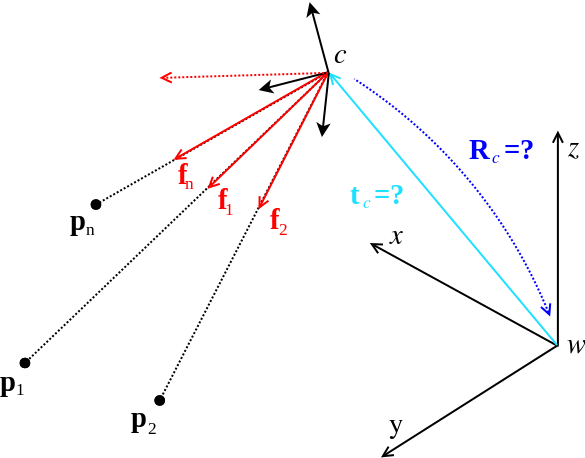
\includegraphics[width=0.6\linewidth]{img/absolute_central.png}
  \caption{From camera frame vectors $f$ (or image pixels if the camera calibration is available) and fix points $p$ the transformation between the two coordinate frames can be computed using the 3pt algorithm. Image from \cite{kneipopengv}}
  \label{fig:img/absolute_centra}
\end{figure}

First, descriptors from every featured point are extracted (both SIFT and SURF can be used updating a configuration file, but in the experiments SIFT will be used). Second, a brute force KNN matching is performed from all the extracted descriptors from on image and all the descriptors of the second image. The first, and second most similar descriptor are retrieved. Then, only good matches are kept, that is, using the matching technique described by Lowe~\cite{lowe2004distinctive}, only matches with a descriptor ratio between the first and the second closest match of 0.8 or less are kept, only discriminant matches are used.\\

Finally, the three-point algorithm is fed with the pixel positions from the query image and the landmarks from the other. Because there are still outliers after the described simple filtering, this process is run in RANSAC~\cite{fischler1981random} framework. \\


\subsubsection{Method validation}
\label{ssub:3pt_method_validation}

Figures~\ref{fig:3pt_matches} and~\ref{fig:3pt_inliers} are an example of the described above. The pose outputted was used to successfully relocalize in SVO.\\

The first part, where descriptors are extracted, matches and filtered, can be seen in Figure~\ref{fig:3pt_matches}.  It can be seen that most matches are correct after this first filtering.\\

The inliers found during the RANSAC process can be seen in~\ref{fig:3pt_inliers}. One has to keep in mind that the model which is fitted  is not from image to image but from world frame, using world points, to camera frame. These world points can not be visualized, only image points, and its precision could lead to not be considered. So some matches which seem right in the image might not be used to calculate the transformation.\\

\begin{figure}[htpb]
  \centering
  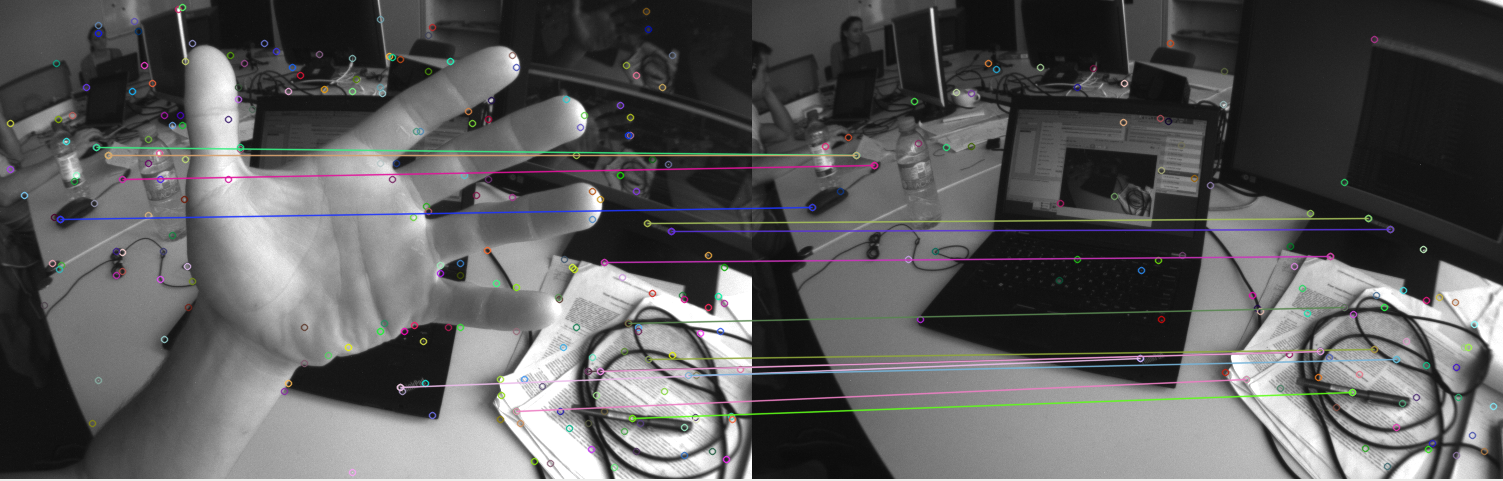
\includegraphics[width=1.0\linewidth]{img/3pt_matches_1.png}
  \caption{Accepted matches using SIFT}
  \label{fig:3pt_matches}
\end{figure}


\begin{figure}[htpb]
  \centering
  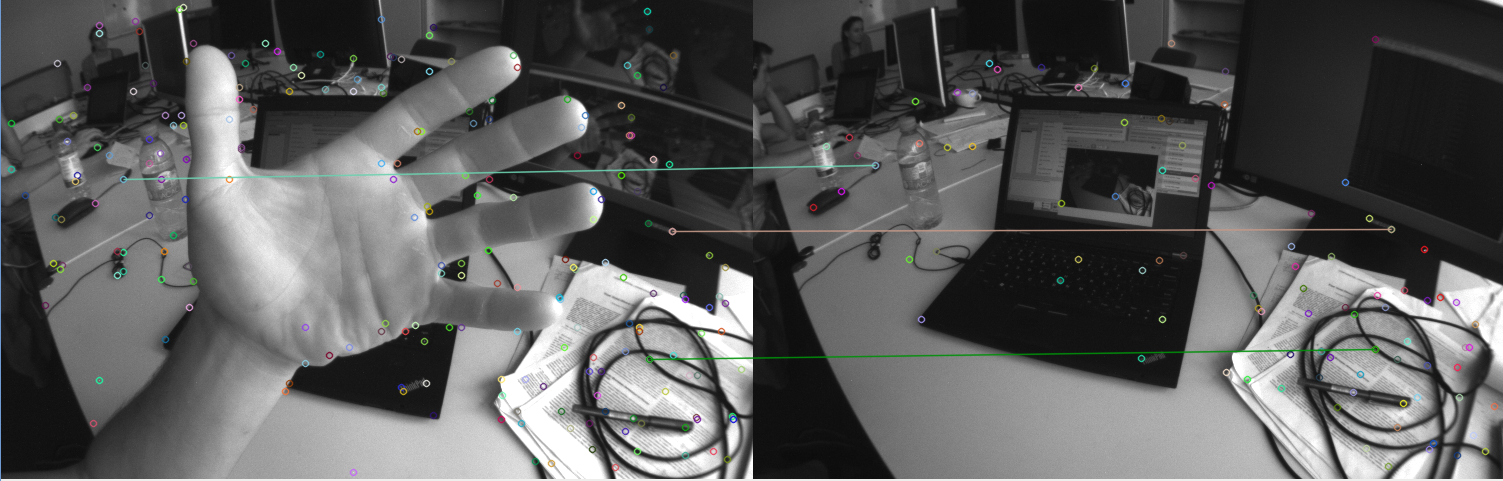
\includegraphics[width=1.0\linewidth]{img/3pt_inliers_1.png}
  \caption{Inliers from RANSAC used to calculate the pose with the three-point algorithm }
  \label{fig:3pt_inliers}
\end{figure}


\section{Using ferns}
\label{sec:using_ferns}

As said previously with the three-point algorithm it is possible to recover the 6 DoF of the camera pose from the relation from pixel coordinates and points in space. In this case machine learning techniques are used to model this relationship. In the classifier scheme, an object in space is a class and multiple views seen from the camera should all be classified as this class.\\

A \textit{fern}~\cite{Ozuysal2010} is a descriptor made from a set of binary tests such as~\ref{eq:fern_test}, build like random forests but flattened (no tree structure). When used as a classifier, every possible evaluation of a \textit{fern} will contain a posterior probability distribution for every class, like random forests' final leafs do.\\

\begin{equation}
  f_j =
  \left\{
    \begin{array}{l l}
      1, & \text{if} \quad I(d_j,1) < I(d_j,2) \\
      0, & \text{otherwise}
    \end{array}
  \right
  \label{eq:fern_test}
\end{equation}

The result of the tests is encoded into the bits of an unsigned integer like done in~\ref{lst:fern_evaluation}. If a \textit{fern} has $S$ tests then its representation can have $K=2^{S}$ possible values which are then used  as index of its posterior distribution.\\

\lstset{language=C++,numbers=none,caption=Fern evaluation, label=lst:fern_evaluation}
\begin{lstlisting}[frame=lines]
uint8_t fern = 0;
for (size_t j = 0; j < S; ++j)
{
  //Shift bits
  fern <<= 1;
  if (I(d_j,1) < I(d_j,2))
  {
    //Change last bit
    fern++;
  }
}
\end{lstlisting}

One \testit{fern} is usually not descriptive enough to correctly classify, in \cite{Ozuysal2010} it is claimed that with 50 \testit{ferns} and $S=11$ a problem with 200 different classes is tractable. In memory, it would involve $50\times2^{11}\times200 = 20480000$ elements to be stored in memory. If these are stored as \textit{float} then 78 MB are needed, which is tractable. It should be noticed that the problem does not scale well on $S$, but at the same time, it is the most critic parameter.\\


\subsection{Seminaive Bayesian Approach}
\label{sub:seminaive_bayesian_approach}

Let $c_i, i = 1,\ldots,H$ be a set of classes and $f_j, j=1,\ldots,N$ be a set of binary tests~\ref{eq:fern_test} calculated over an image patch that is being classified. Formally, we are looking for

\begin{equation}
  \^c_i = \underset{c_i}{\text{argmax}} \quad P(C = c_i | f_1, f_2, \ldots, f_N)
\end{equation}

then, Bayes' formula tells

\begin{equation}
  P(C = c_i | f_1, f_2, \ldots, f_N) = \frac{P(f_1,f_2,\ldots,f_N \arrowvert C=c_i) P(C=c_i)}{P(f_1,f_2,\ldots,f_N)}
\end{equation}

Assuming a uniform prior and since the denominator is a scaling factor the problem is reduced to

\begin{equation}
  \^c_i = \underset{c_i}{\text{argmax}} \quad P(f_1, f_2, \ldots, f_N | C = c_i)
\end{equation}

Since these tests are very simple, many of them are needed ($N \approx 300$), the storage of joint probabilities for every outcome is no feasible because $2^N$ entries for each class would be required. One way to avoid this storage is to assume total independence between tests, this way the class probability distributions can be calculated like

\begin{equation}
  P(f_1, f_2, \ldots, f_N | C = c_i) = \prod^{N}_{j=1}P(f_j | C = c_i)
\end{equation}

but this ignores the possible correlation between tests. With \testit{ferns} a trade off is achieved, tests are grouped in sets $F$ and then the conditional probability becomes

\begin{equation}
  P(f_1, f_2, \ldots, f_N | C = c_i) = \prod^{M}_{k=1} P(F_k | C = c_i)
\end{equation}

It can be seen here why $S$ is important, an increment in the number of tests in a \textit{fern} means an increment in the modelled correlation.\\

\subsection{Training}
\label{sub:training}

During the training step many different views of a world point are needed to correctly model it. In the original work \cite{Ozuysal2010} only one image is used to train and to generate more possible views of the objects multiple (about 10,000) randomly generated warps are applied to it, all this warped images are used for training. Those warps include affine transformations, noise addition and smoothing with a Gaussian kernel (with all the parameters randomly picked from a uniform distribution).\\

In the studied case here, the algorithm can already provide multiple real views of the object (around 5-10), but still on each patch many randomly generated warps are applied and used to train (usually 100). In this case, the warps are simplified to include only image rotation and scale.\\

During the training, every warped patch is evaluated with every \textit{fern}. The count of a class evaluation on each \textit{fern} is performed along with the count of per class patches used. Those values are used during the classification step to calculate the probability distributions

\begin{equation}
  p_{k,c_i} = \frac{N_{k,c_i} + N_r}{N_{c_i} + K \times N_r}
\end{equation}

where $N_{k,c_i}$ is the number views of class $c_i$ that evaluates to $k$ and $N_{c_i}$ is the number of views of class $c_i$ to train. A regularization term $N_r = 1$ is used to avoid probabilities evaluating to zero. The implemented classifier sores $c_i$  and $N_{k,c_i}$, allowing online training by evaluating new incoming images and featured points.\\

In the current implementation no online training is performed because training one frame is already computationally expensive and it cannot be done at every new keyframe from SVO without drastically lowering the amount of frames treated per second. Instead one global training is triggered manually when it cannot disturb the MAV's flight, for example when landed. Online training could be implemented on a different tread if the used board has unused cores.\\


\subsubsection{Method Validation}
\label{ssub:ferns_method_validation}

To validate the classifier a small test has been set up. One image is taken and from it 100 random patches are used to train the classifier. Then, 100 random warps are applied to each one these patches and are classified. This process is reproduced 100 times because it is a random process. The ratio of well classified warped patches with contrast to the number of \textit{ferns} used and the number of tests per \textit{fern} can be seen in the next plot.


\begin{figure}[htpb]

  \centering
  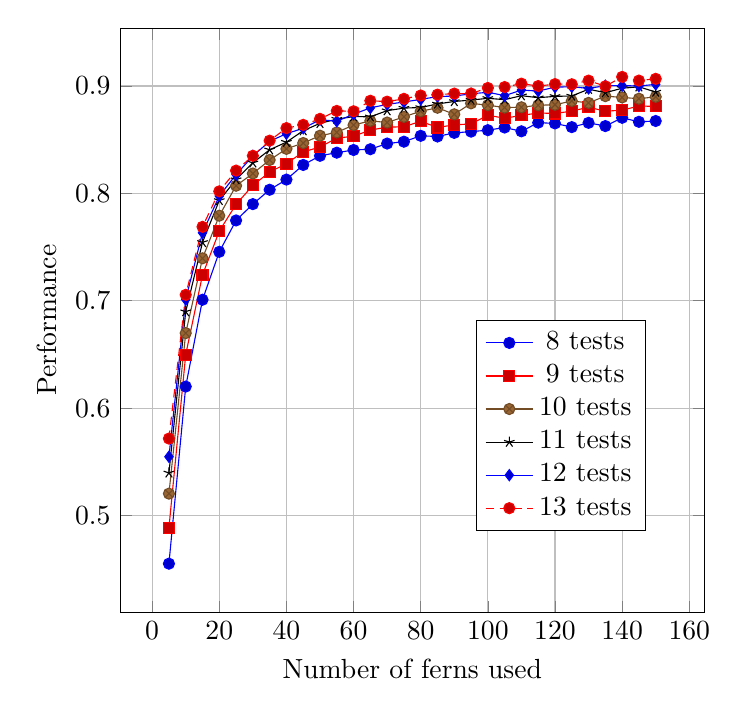
\begin{tikzpicture}
  \begin{axis}[
  height=9cm,
  width=9cm,
  grid=major,
  xlabel=Number of ferns used,
  ylabel=Performance,
  legend style = {
    at={(0.9,0.5)}
  }
  ]

  \addplot coordinates
  {
  (5,0.455156)
  (10,0.620105)
  (15,0.700959)
  (20,0.745575)
  (25,0.774825)
  (30,0.790016)
  (35,0.803403)
  (40,0.812852)
  (45,0.826499)
  (50,0.835003)
  (55,0.837928)
  (60,0.840413)
  (65,0.841138)
  (70,0.846428)
  (75,0.848151)
  (80,0.85363)
  (85,0.853007)
  (90,0.856371)
  (95,0.857518)
  (100,0.858881)
  (105,0.861345)
  (110,0.857811)
  (115,0.865893)
  (120,0.865168)
  (125,0.861729)
  (130,0.865707)
  (135,0.862695)
  (140,0.870416)
  (145,0.866652)
  (150,0.867423)
  };
  \addlegendentry{8 tests}

  \addplot coordinates
  {
  (5,0.488611)
  (10,0.649876)
  (15,0.724042)
  (20,0.76488)
  (25,0.789768)
  (30,0.807459)
  (35,0.819871)
  (40,0.827699)
  (45,0.838572)
  (50,0.843236)
  (55,0.851409)
  (60,0.853273)
  (65,0.858985)
  (70,0.86166)
  (75,0.862066)
  (80,0.867132)
  (85,0.861412)
  (90,0.86384)
  (95,0.864704)
  (100,0.872822)
  (105,0.869988)
  (110,0.87266)
  (115,0.874865)
  (120,0.874463)
  (125,0.876594)
  (130,0.880322)
  (135,0.876503)
  (140,0.877519)
  (145,0.881349)
  (150,0.88105)
  };
  \addlegendentry{ 9 tests}

  \addplot coordinates
  {
  (5,0.520388)
  (10,0.669885)
  (15,0.73953)
  (20,0.779234)
  (25,0.807139)
  (30,0.81853)
  (35,0.831105)
  (40,0.841473)
  (45,0.846916)
  (50,0.853759)
  (55,0.85682)
  (60,0.863666)
  (65,0.867547)
  (70,0.866015)
  (75,0.87127)
  (80,0.876509)
  (85,0.879735)
  (90,0.873673)
  (95,0.883855)
  (100,0.882149)
  (105,0.879932)
  (110,0.88022)
  (115,0.882092)
  (120,0.882542)
  (125,0.886073)
  (130,0.884312)
  (135,0.890578)
  (140,0.889372)
  (145,0.888186)
  (150,0.889946)
  };
  \addlegendentry{10 tests}

  \addplot coordinates
  {
  (5,0.539702)
  (10,0.689876)
  (15,0.754419)
  (20,0.793475)
  (25,0.812848)
  (30,0.828437)
  (35,0.84063)
  (40,0.847733)
  (45,0.858395)
  (50,0.865242)
  (55,0.869159)
  (60,0.871521)
  (65,0.871361)
  (70,0.877042)
  (75,0.879435)
  (80,0.880008)
  (85,0.883295)
  (90,0.885611)
  (95,0.886914)
  (100,0.888524)
  (105,0.887305)
  (110,0.89099)
  (115,0.889118)
  (120,0.890359)
  (125,0.890729)
  (130,0.897019)
  (135,0.893813)
  (140,0.897917)
  (145,0.899281)
  (150,0.89439)
  };
  \addlegendentry{11 tests}

  \addplot coordinates
  {
  (5,0.554762)
  (10,0.701209)
  (15,0.763357)
  (20,0.797581)
  (25,0.817505)
  (30,0.834899)
  (35,0.848518)
  (40,0.855628)
  (45,0.860604)
  (50,0.868656)
  (55,0.867211)
  (60,0.873718)
  (65,0.879655)
  (70,0.882888)
  (75,0.885119)
  (80,0.887547)
  (85,0.890143)
  (90,0.890705)
  (95,0.892726)
  (100,0.894182)
  (105,0.891051)
  (110,0.896253)
  (115,0.895273)
  (120,0.898981)
  (125,0.899296)
  (130,0.897772)
  (135,0.900302)
  (140,0.900423)
  (145,0.899991)
  (150,0.901546)
  };
  \addlegendentry{12 tests}

  \addplot coordinates
  {
  (5,0.571666)
  (10,0.705516)
  (15,0.768864)
  (20,0.801934)
  (25,0.821235)
  (30,0.835033)
  (35,0.849129)
  (40,0.860822)
  (45,0.863828)
  (50,0.869423)
  (55,0.876834)
  (60,0.876493)
  (65,0.886291)
  (70,0.885457)
  (75,0.888078)
  (80,0.891203)
  (85,0.891976)
  (90,0.892937)
  (95,0.893008)
  (100,0.898195)
  (105,0.899039)
  (110,0.902219)
  (115,0.899978)
  (120,0.901776)
  (125,0.901647)
  (130,0.905039)
  (135,0.899778)
  (140,0.908492)
  (145,0.905066)
  (150,0.906713)
  };
  \addlegendentry{13 tests}

  \end{axis}
  \end{tikzpicture}
  \caption{Ferns classifier evaluation}
  \label{fig:ferns_classifier_evaluation}
\end{figure}

It can be seen that a minimum number of \textit{ferns} is needed to achieve the best performance for a given number of tests, between 50 and. After that, more tests cannot improve the results. On the other side, it can be seen that incrementing the number of tests per \textit{fern} can give a qualitative jump, even with only one test. As said before, the number of tests $S$ is an important parameter, but it is very limited by memory.\\
